\subsection{Alternative losses and activations}

The choice of loss functions and activations in deep networks has a significant effect on the training dynamics and task performance.

\subsubsection{Definitions}

Foothill function \citep{belbahri2019foothill} is defined as

\begin{align}
    p_{\alpha,\beta}(x) = \alpha x~ \mathrm{tanh}\left( \frac{\beta x}{2} \right).
    \label{eq:reswish}
\end{align}

where $\mathrm{tanh}(.)$ is the hyperbolic tangent function, $\alpha > 0$ is a shape parameter and $\beta > 0$ is a scale parameter. % and $\mu$ a location parameter. 
The function is symmetric about $0$ (see Figure \ref{fig:foothill}, left panel). The first and the second derivatives (see Figure \ref{fig:foothill}, right panel) of foothill are 

\begin{align*}
    \frac{dp_{\alpha,\beta}(x)}{dx} = \alpha ~ \mathrm{tanh}\left( \frac{\beta x}{2} \right) + \frac{1}{2} \alpha \beta x ~ \mathrm{sech}^2\left( \frac{\beta x}{2} \right), \\
     \frac{d^2p_{\alpha,\beta}(x)}{d^2x} = \frac{1}{2} \alpha \beta~ \mathrm{sech}^2\left( \frac{\beta x}{2} \right) \left\{  2 - \beta x ~ \mathrm{tanh}\left( \frac{\beta x}{2} \right) \right\},
\end{align*}
where $\mathrm{sech}(.)$ is the hyperbolic secant function.

\begin{figure}[htb]
    \centering
    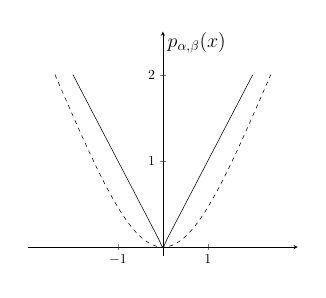
\begin{tikzpicture}[scale=0.5]
    \begin{axis}[
      axis x line=middle, axis y line=middle, samples = 200,
      ylabel={$p_{\alpha,\beta}(x)$},ylabel style={font=\Large, yshift=3pt},
      ymin=-0.1, ymax=2.5, ytick={0,1,2},
      xmin=-3, xmax=3, xtick={-1, 0, 1}
    ]
    \addplot[black, domain=-2.4:2.4, dashed]{1*2*(x-0)*((1+pow(e,-1*(x-0)))^(-1) - 0.5)};
    \addplot[black, domain=-2:2, smooth]{1*2*(x-0)*((1+pow(e,-50*(x-0)))^(-1) - 0.5)};
    \end{axis}
    \end{tikzpicture} 
    \hspace{0.5cm}% NO SPACE!
    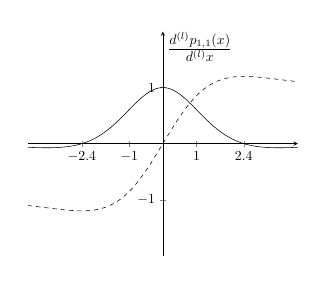
\begin{tikzpicture}[scale=0.5]
            \begin{axis}[
      axis x line=middle, axis y line=middle, samples = 100,  ylabel={$\frac{d^{(l)}p_{1,1}(x)}{d^{(l)}x}$},ylabel style={font=\Large, yshift=3pt}, ymin=-2, ymax=2, ytick={-1,0,1}, xtick={-2.4, -1, 0, 1, 2.4},
      xmin=-4, xmax=4
    ]
    \addplot[black, domain=-4:4, dashed]{2*(1+pow(e,-1*x))^(-1)*(1+1*x*pow(e,-1*x)*(1+pow(e,-1*x))^(-1)))-1};
    \addplot[black, domain=-4:4, smooth]{2 * (-1^2 * x * pow(e, -1*x) * (1+pow(e,-1*x))^(-2) + 2 * 1^2 * x * pow(e, -2*1*x) * (1+pow(e,-1*x))^(-3) + 2 * 1 * pow(e, -1*x) * (1+pow(e,-1*x))^(-2)) };
    \end{axis}
    \end{tikzpicture} 
    \caption{Left panel: Regularization function \eqref{eq:reswish} for $\alpha=1$, $\beta=1$ (solid line)  and $\alpha=1$, $\beta = 50$ (dashed line). Right panel: The first (dashed line) and the second (solid line) derivatives of the regularization function \eqref{eq:reswish} for $\alpha=1$ and $\beta=1$.
    }
    \label{fig:foothill}
\end{figure}

\subsubsection{Properties}

The regularization function (\ref{eq:reswish}) has several interesting properties. It is infinitely differentiable and symmetric about the origin, $$ p_{\alpha,\beta}(x) =  p_{\alpha,\beta}(-x).$$ 
Also, it is flexible enough to approximate the lasso \cite{Tibshirani_lasso_1996} and Ridge penalties \cite{hoerl1970ridge} for particular values of $\alpha$ and $\beta$. The following properties suggest that this function could be considered as a quasiconvex alternative to the elastic net penalty \cite{zou2005regularization}.

\begin{property}  For $\alpha=1$ and $\beta \rightarrow \infty$, the foothill penalty (\ref{eq:reswish}) converges to the lasso penalty.
\end{property}

\emph{Proof.} For $x>0$, it is easy to see that
\begin{flalign*}
    \lim_{\beta \rightarrow +\infty}& \mathrm{tanh}\left( \frac{\beta x}{2} \right) = 1,\\
	\lim_{\beta \rightarrow +\infty}& p_{\alpha, \beta}(x) = x.
\end{flalign*}

Equivalently, for negative $x$, as $p_{\alpha, \beta}(x)$ is symmetric about the origin, then $\lim_{\beta \rightarrow +\infty} p_{\alpha, \beta}(x) = -x$, which is equivalent to $p_{\alpha, \beta}(x) \rightarrow |x|$ when $\beta \rightarrow +\infty$.

\begin{property}  For $\alpha>0$, $\beta>0$, and $\beta = 2 / \alpha$ the foothill penalty  (\ref{eq:reswish}) approximates the Ridge penalty in a given interval $[-c ; c]$.
\end{property}

\emph{Proof.} Let us study this property formally. Take the Taylor expansion of (\ref{eq:reswish}), 
\begin{align}
    p_{\alpha, \beta}(x) \approx \frac{\alpha\beta}{2} x^2 - \frac{\alpha\beta^3}{24} x^4 + \frac{\alpha\beta^5}{240} x^6 + \mathrm{O}(x^8).
	\label{eq:taylor}
\end{align}

And, for a given $c>0$, 
\begin{align}
    \int_{0}^{c} \left( \frac{\alpha\beta}{2} x^2 - p_{\alpha, \beta}(x)  \right)^2 dx \approx \frac{\alpha^2\beta^6}{5184} c^9 + \mathrm{O}(c^{11}).
	\label{eq:approxridge}
\end{align}

The integral in (\ref{eq:approxridge}) diverges if $c$ tends to infinity, but for a finite positive number $c$, one can numerically estimate the minimal distance between the $L_2$ norm and (\ref{eq:reswish}) with a tiny approximation error. This can be achieved by taking $\beta = 2 / \alpha$ and (\ref{eq:approxridge}) becomes 
\begin{align}
    \int_{0}^{c} \left( x^2 - p_{\alpha, \beta}(x)  \right)^2 dx \approx \frac{1}{81\alpha^4} c^9 + \mathrm{O}(c^{11}) = \varepsilon_c .
	\label{eq:approxridge2}
\end{align}
For large values of $\alpha$, the error $\varepsilon_c$ is negligible, see for example Figure \ref{fig:approxridge} where the regularization function (\ref{eq:reswish}) approximates the Ridge penalty almost perfectly within $[-5 ; 5]$. Furthermore, for fixed parameters, note that 
\begin{align*}
    \lim_{x \rightarrow +\infty} p_{\alpha, \beta}(x) - \alpha x = 0, ~~\mathrm{and}~~  
	\lim_{x \rightarrow -\infty} p_{\alpha, \beta}(x) + \alpha x = 0.
\end{align*}

Hence it is also interesting to note that (\ref{eq:reswish}) behaves like a polynomial function for small values of $x$, and like a linear function for large values. Therefore, using it as a loss function (instead of a regularization), (\ref{eq:reswish}) behaves like the Huber loss used in practice for robust estimation \cite{huber1964robust}. Figure \ref{fig:approxridge} shows that (\ref{eq:reswish}) is bounded between the Huber loss and the squared error loss.

\begin{figure}[htb]
    \centering
    \includegraphics[scale=0.4]{figures/fig/huber_like_foothill.pdf} 
    \caption{Plots of the Ridge, the foothill penalty with $\alpha = 16$ and $\beta=0.125$ and twice the Huber loss. The solid blue line represents the foothill penalty, the dashed line represents the Ridge one (upper bound) and Huber (lower bound) is represented in dotted line.}
    \label{fig:approxridge}
\end{figure}

\begin{property}  Saddle points of $p_{\alpha, \beta}(x)$ are $x_0 \approx \pm 2.3994/\beta$ and $p_{\alpha, \beta}(x_0) = \frac{2 \alpha }{\beta}$.
\end{property}

\emph{Proof.} Indeed, the second order derivative vanishes at
\begin{align*}
     2 - \beta x ~ \mathrm{tanh}\left( \frac{\beta x}{2} \right) = 0,\\
\end{align*}
which is solved by an iterative method for  $\beta x \approx \pm 2.3994$. This implies
\begin{align*}
     \beta x_0 ~ \mathrm{tanh}\left( \frac{\beta x_0}{2} \right) = 2,
\end{align*}
or equivalently
\begin{align*}
	p_{\alpha, \beta}(x_0) = \frac{2 \alpha }{\beta}.
\end{align*}

\begin{property}  The function $p_{\alpha, \beta}(x)$ is quasiconvex.
\end{property}

\emph{Proof.} It is straight forward to show that $p_{\alpha, \beta}(x)$ is decreasing from $-\infty$ to $0$ and increasing from $0$ to $+\infty$ and any monotonic function is quasiconvex (see Figure \ref{fig:foothill}, right panel).



\vspace{0.5cm}
Table \ref{tab:relation} suggests that foothill has the flexibility to be used for feature selection regularizer such as the lasso or used only to shrink the estimator in order to prevent over-fitting like the Ridge. Finally, it also can be used as a loss function for robust regression as an alternative to the Huber loss.

\begin{table}[htb]
\caption{Relationship to other functions} \label{tab:relation}
\begin{center}
\begin{tabular}{l@{\hspace{0.1in}}l@{\hspace{0.1in}}l@{\hspace{0.1in}}l}
  & Shape $\alpha$ & Scale $\beta$ & Function\\
\hline
Lasso        & $1$ & $+\infty$  & $p_{\alpha, \beta}(x)=|x|$\\
Ridge        & $+\infty$ & $2 / \alpha$ & $p_{\alpha, \beta}(x)=x^2$\\
Huber & $< +\infty$ & $2 / \alpha$ &  $p_{\alpha,\beta}(x) = \alpha x~ \mathrm{tanh}\left( \frac{x}{\alpha} \right)$\\
Foothill   & $1$ & $2$ & $p_{\alpha, \beta}(x)=x \mathrm{tanh}(x)$\\
\end{tabular}
\end{center}
\end{table}
